\documentclass[UTF8]{ctexrep}

\usepackage{fontspec}
\usepackage{graphicx}

%--------------------------%

% \setmonofont{Consolas}
\ctexset{
    section/name = {第,节},
    section/number = {\arabic{section}},
    subsection/number = {\arabic{section}.\arabic{subsection}}
}

\title{郑和后台计划}
\author{zcy}

\bibliographystyle{acm}

\begin{document}
\maketitle
\newpage


%--------------------------%
\begin{figure}[h]
    \caption{整体架构}
    \centering
    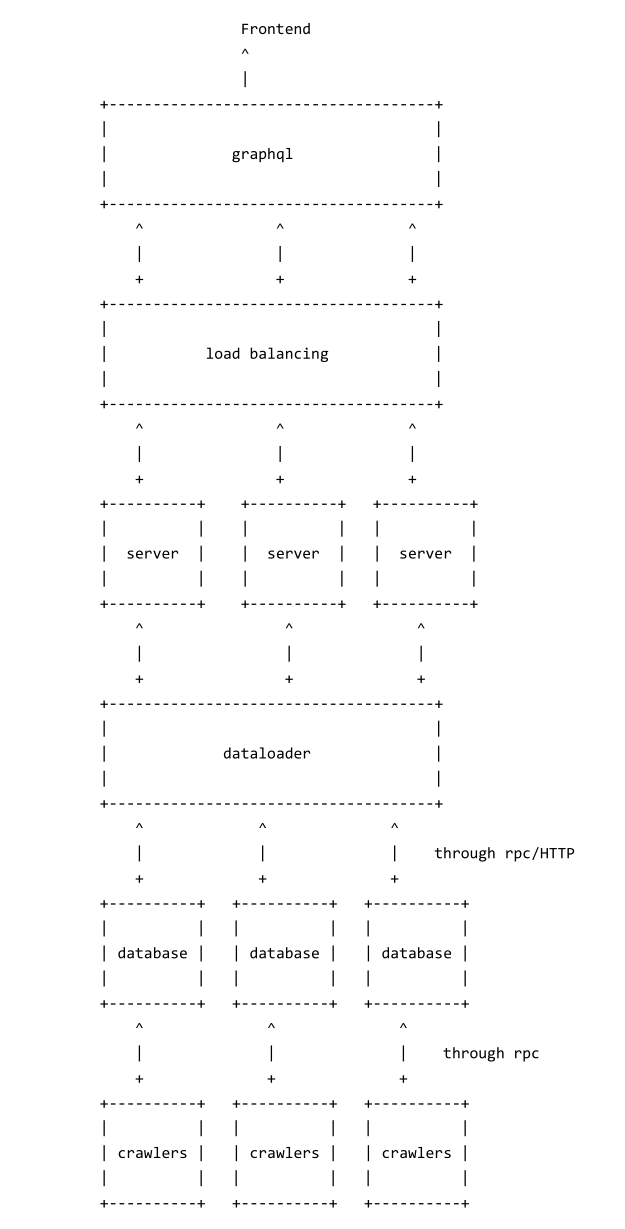
\includegraphics[width=0.75\textwidth]{assets/figures/arch2.png}
    \label{fig:arch}
\end{figure}

\part{数据获取}

\subsection{使用scrapy方案}

\paragraph{scrapy特点}
\begin{itemize}
    \item scrapy 是一个使用python,未来爬取网站数据,提取数据而编写的应用框架,具有模块化特点。因此只需要几个模块就可以实现爬虫。
\end{itemize}
\par

\paragraph{scrapy模块(主要)}

\begin{itemize}
    \item scrapy engine 负责Spider、ItemPipeline、Downloader、Scheduler中间的通讯,信号、数据传递等。

    \item Scheduler: 它负责接受引擎发送过来的Request请求,并按照一定的方式进行整理排列,入队,当引擎需要时,交还给引擎。
    
    \item Downloader:负责下载Scrapy Engine(引擎)发送的所有Requests请求,并将其获取到的Responses交还给Scrapy Engine(引擎),由引擎交给Spider来处理。
    
    \item Spider:它负责处理所有Responses,从中分析提取数据,获取Item字段需要的数据,并将需要跟进的URL提交给引擎,再次进入Scheduler(调度器)。
    
    \item Item Pipeline:它负责处理Spider中获取到的Item,并进行进行后期处理(详细分析、过滤、存储等)的地方。
\end{itemize}
\par

\paragraph{意义}
\begin{itemize}
    \item 开发迅速:一般情况下,只需要对其中的spider, pipeline进行编写。

    \item 适应多网站爬取:爬取数据主要由spider进行,如果需要对多个网站进行爬取,可以在同一个项目中快速新建爬虫而不需要修改Pipeline。因而未必需要通用爬虫。
    
    \item 弹性高:易于进行二次调整。
\end{itemize}
\par

\subsection{item}
\begin{itemize}
    

    \item 此处由杨澍生学长和王清雨大佬达成了对接,目前没有改变。

    \item 由于要使用二进制传输,所以不需要对item进行编写,只要将data从spider传到pipeline并进行打包item。
    
    \item 对这个item内容的修改,需要在pipline和sipder进行微调,不需要对item.py进行修改。
    
    \item 基于数据库需求的详细要求也由学长完成。
\end{itemize}

\paragraph{paper}
\textit{protobuf repeated类型相当于std的vector,可以用来存放N个相同类型的内容。}
\begin{verbatim}
    string title = 1;
    string journal = 2;
    string journal_name = 3;
    repeated string author = 4;
    string date = 5;
    string pagination = 6;
    string issueNumber = 7;
    string volumeNumber = 8;
    string genre = 9;
\end{verbatim}
\par

\paragraph{person}
\begin{verbatim}
    string name = 1;
    repeated Paper paper = 2;
\end{verbatim}
\par

\paragraph{spider}
杨澍生学长之前已经完成了对dblp的爬虫编写,提供了很好的范本,但是没有实现多网站的爬取。
王清雨大佬提供的后台方案中,只需要对爬取的数据打包成Item直接存储即可。
\par

\paragraph{未来需要完成的方案}
\begin{itemize}
    \item 根据需求,完成多个网站的spider爬虫编写。

    \item 找出paper页面的一般规律,并确保能爬取一个网站的全部内容或者从单一不重复的列表中获取内容。\textit{若能够比较成功地查找url的规律,就可以构造start\_urls来确保内容不被重复爬取。对于能够获得单一不重复列表(例如DBLP)的网站可以采用此方案。}
    
    \item 对于不能找出一般规律的,可以使用半通用爬虫,使用正则表达式或者通过item进行判断是否符合需求(比如item中发表期刊是否为计算机类型),递归爬取网站全部页面并提取所需要的内容。\textit{此处要对需要爬取的网站进行调研。}\textit{此处使用正则表达式爬取的内容可能会出现数据错误率的问题,因而半通用爬虫可能需要清洗。}
    
    \item 定期进行重新爬取网站全部内容,并与数据库进行更新。\textit{此处考虑可以使用增量爬虫,但是增量爬虫需要两个数据库配合,并且增量爬虫具有内存爆炸的问题,目前只做实验考虑。}
    
    \item (可能需要)构建ip池,对一些可能封杀Ip的网站使用。
\end{itemize}
\par

\subsection{pipline}

\textit{数据库使用protobuf, 因此,只要将爬取的数据加工后直接写入即可。此前, 杨澍生学长的爬虫已经完成了对数据地加工。}

\paragraph{未来需要完成的部分}
\begin{itemize}
\item 利用新的接口,将爬虫数据自动写入数据库。
\end{itemize}

\subsection{总结和展望}
\begin{itemize}
    \item  下一步是完成对多个网站数据的爬取。

    \item  在学长的基础上,这个目标能够比较快的实现。
    
    \item  需要加强对爬虫相关知识(包括爬虫)的学习,此外,有一些新的内容需要实现需要努力。
\end{itemize}


%--------------------------%

\part{数据存储}

\section{与爬虫对接}

\paragraph{需求分析}

需要约定接口,对获取到的数据类型及内容进行约束。

\paragraph{Protocal Buffer}

是著名科技公司\textmd{Google}提出的与语言无关,与平台无关,可扩展的用于序列化结构化数据的机制,类似\texttt{XML}和\texttt{JSON}但更简单也更快速。

\par
通过定义\texttt{.proto}的接口文件,规定好需要存储的数据的类型、结构、大小等,更方便进行存储。

\paragraph{RPC}

同样通过\texttt{Protobuf}定义\texttt{RPC Service}需要的参数与格式,供爬虫方调用。

\paragraph{可能存在的问题}

\begin{itemize}
    \item 爬虫获取到不在定义中的数据
    \item 新的数据与已有数据重复或冲突
    \item 存储失败后如何重新存储
\end{itemize}

\section{数据库的选择}

\paragraph{需求分析}

存储需要做到:
\begin{itemize}
    \item 体现数据之间的关联
    \item 可扩展性高
    \item 可存储的数据量大
    \item 根据数据间的联系快速搜索
\end{itemize}

因此我们选用了图数据库\texttt{Dgraph}\footnote{https://dgraph.io}作为存储数据库。

\paragraph{特点}

\texttt{Dgraph}具有以下特点:

\begin{itemize}
    \item 分布式——可以部署在多台服务器上,减轻服务器压力
    \item 快速——能快速对查询进行相应
    \item 高可用性——自动进行同步复制,重启失败的实例
    \item 事务支持——保证数据的一致性
    \item 灵活——随时可调整数据的模式
\end{itemize}

\paragraph{存在的问题}

首先,查询语句不够成熟。
\par
采用了一套自定义的查询语句,不易维护,且语法较为晦涩
\par
其次,该项目比较年轻,不稳定。

\paragraph{主库与从库}

由于需要对获取来的数据进行整合、聚类、分析等准备工作,因此设置\emph{主库与从库},主库中为已经经过处理过的数据,主要用来给用户展示等。而爬虫获取到的数据则直接写入从库,经过处理后再统一与主库进行合并。

\par

采用主库与从库分离的方式,一方面方便对数据的分析与整理;另一方面由主库主要负责读操作、从库主要负责写操作,减轻同时读写对数据库带来的压力。

\paragraph{可能存在的问题}

\begin{itemize}
    \item 如何正确地合并两个库
    \item 如何保证数据一致性、不丢失
    \item 如何从从库中获取数据并异步处理
\end{itemize}

%--------------------------%

\part{数据搜索}

\section{两大需求}

Aminer 提供快速,精确的搜索服务。以学者搜索为例,系统会按照学者的论文数、被引用数、h-index等指标排序并且能准确地区分\textbf{同名}的不同学者。

而在论文搜索中,Aminer 不仅仅能根据文章名进行搜索,还可以搜索与某一特定主题对应的论文。例如:直接搜索\textit{Data Mining}就会出现数据挖掘领域的杰出论文。\\

因此,郑和平台目前最主要的两个需求如下:

\begin{itemize}
    \item 根据关键词检索相关学者
    \item 根据关键词检索相关论文
\end{itemize}

考虑到用户体验和搜索结果的呈现质量,下述章节将基于这两大需求进行更为细致的分析,同时提供相应的解决方案。

\section{关键词预处理}

在查询数据库之前,至少应对用户输入进行如下处理:

\begin{itemize}
    \item 对用户输入内容的容错(例如拼写错误或输入错误)
    \item 对同义词、近义词的处理
    \item 对词型变化及格位变化的处理(词干提取)
    \item 分词
\end{itemize}

上述大部分都或多或少地与NLP相关。在项目开始的初期(目前),我们考虑使用成熟的开源实现。

\subsection{用户输入容错}

从后端方向考虑,郑和平台所采用的图数据库内建对Fuzzy Search的支持,但需要建立相应的特殊索引。

\subsection{同义词与近义词}

基于Word2Vec的实现方式,进行同义词识别。\\

同时列出一些较为流行的开源实现以供参考:

\begin{itemize}
    \item Synonyms\footnote{https://github.com/huyingxi/Synonyms},预训练的中文相关词汇实现
    \item wordvectors\footnote{https://github.com/Kyubyong/wordvectors},支持多语言的Word2Vec实现
\end{itemize}

\subsection{分词}

英文语境下的分词依照空格分割之后去除介词和代词。

若来自用户的中文输入为句子(考虑到并非所有用户会用分隔符将关键词分开),首先应进行分词。

开源社区已有极为优秀和高效的中文分词实现jieba\footnote{https://github.com/fxsjy/jieba},具有如下优势:

\begin{itemize}
    \item 基于前缀词典实现高效的词图扫描,生成句子中汉字所有可能成词情况所构成的有向无环图 (DAG)
    \item 采用了动态规划查找最大概率路径, 找出基于词频的最大切分组合
    \item 对于未登录词,采用了基于汉字成词能力的 HMM 模型,使用了 Viterbi 算法
\end{itemize}

\subsection{词干提取}

相比分词,在中文语境下对用户输入进行词干提取的实用意义不是很大(直觉得出,尚无数据佐证)。

而在英文语境下,对关键词进行词干提取是必要的。例如,以关键词“optimization”和“optimized”分别进行搜索被期待返回接近或者相同的查询结果。事实上,Google和Bing等搜索引擎确实对用户输入进行了词干提取。

采用Porter算法\cite{porter2006algorithm}进行词干提取效果较好,论文作者同时提供了免费的改进项目Snowball\footnote{https://snowballstem.org/}。

\section{权重与优先级}

对于每次搜索,用户输入经过预处理后应具有类似如下的结构:

$$i=\{p,\ p[\ ],\ s[\ ],\ r[\ ]\}$$

$p$为用户的原始输入字符串,$p[\ ]$为分词结果,$s[\ ]$为词干提取结果,$r[\ ]$为相关词汇。

对$i$中每个元素赋予不同的权重$w_n$,依据$\sum{w_n}$决定搜索结果的相关程度。具体权重的分配方法仍需进一步讨论。

\section{搜索词频统计}

在数据库层面进行持久化,对每次搜索过程的分词结果$p[\ ]$和词干提取结果$s[\ ]$进行索引。

定期分析搜索日志,进行进一步分析(?)

\section{热点数据缓存}

为减轻服务器压力,应基于搜索词频统计结果,将热点数据缓存。

详见数据库部分。

%--------------------------%

\bibliography{papers}

%--------------------------%

\end{document}
